\documentclass[alsotrans]{beamerswitch}
\usepackage{sdp}

\title{Списък}

\date{28 октомври 2019 г.}

\titlegraphicx{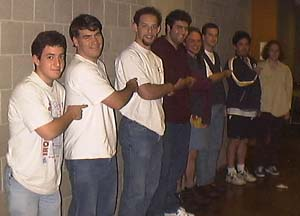
\includegraphics[height=0.25\textheight]{images/list.jpg}\\
 \imageUntitledAttr{Prettysleepy2}{https://pixabay.com/images/id-3517582/}{Pixabay License}}

\begin{document}

\begin{frame}
  \titlepage
\end{frame}

\section{АТД списък}

\begin{frame}
  \frametitle{АТД: списък}

  Хомогенна линейна структура с последователен достъп до елементите\\[2ex]
  Операции:\\[1ex]
  \begin{itemize}
  \item \tt{create()} --- създаване на празен списък
  \item \tt{empty()} --- проверка за празен списък
  \item \tt{insert(x, p)} --- включване на елемент \tt x на дадена позиция \tt p
  \item \tt{delete(p)} --- изключване на елемент на дадена позиция \tt p
  \item \tt{get(p)} --- достъп до елемент на дадена позиция \tt p
  \end{itemize}
\end{frame}

\begin{frame}
  \frametitle{Едносвързано представяне}

  \begin{center}
    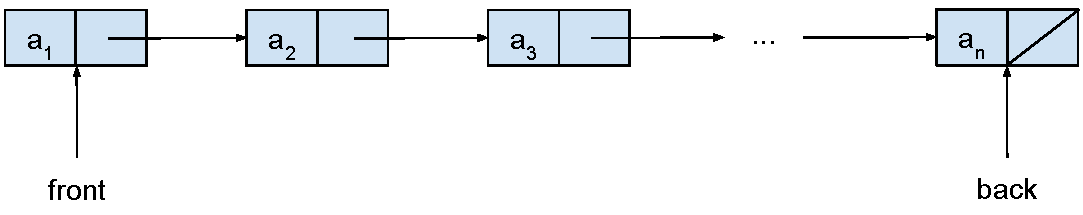
\includegraphics[width=\textwidth]{images/linked_list.pdf}
  \end{center}
\end{frame}

\begin{frame}
  \frametitle{Едносвързано циклично представяне}

  \begin{center}
    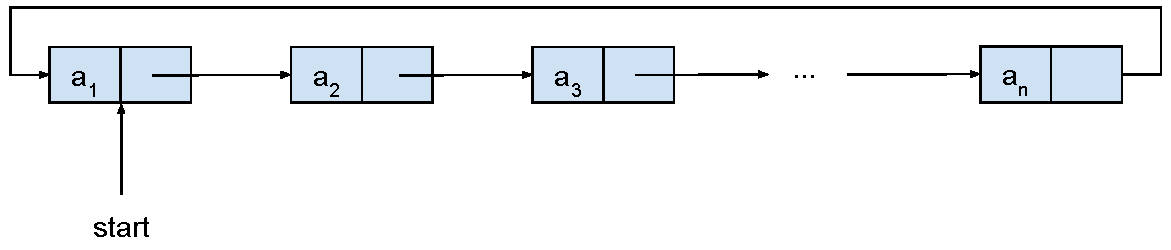
\includegraphics[width=\textwidth]{images/linked_cyclic_list.pdf}
  \end{center}
\end{frame}

\begin{frame}[label=doublelinked]
  \frametitle{Двусвързано представяне}

  \begin{center}
    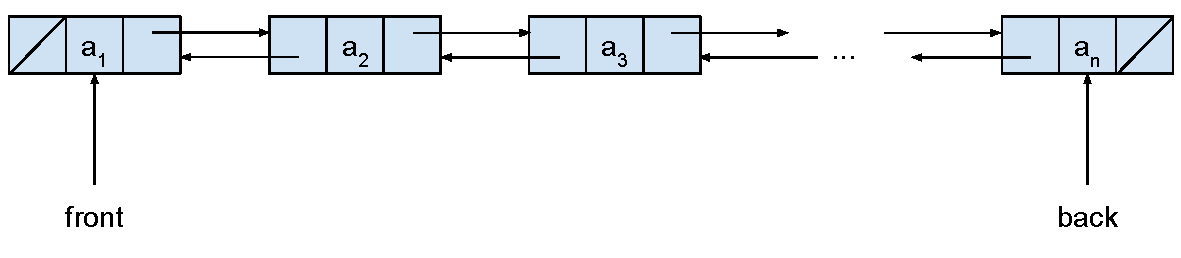
\includegraphics[width=\textwidth]{images/double_linked_list.pdf}
  \end{center}
\end{frame}

\begin{frame}
  \frametitle{Двусвързано циклично представяне}

  \begin{center}
    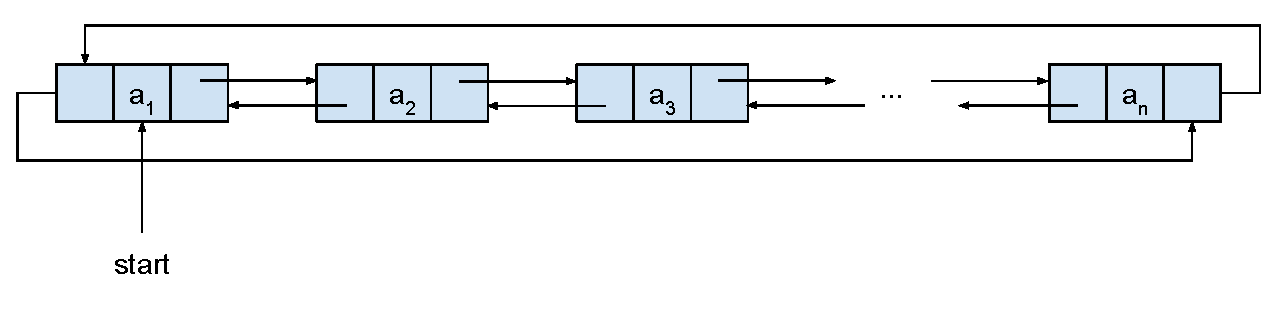
\includegraphics[width=\textwidth]{images/double_linked_cyclic_list.pdf}
  \end{center}
\end{frame}

\section{Итератори}

\begin{frame}
  \frametitle{АТД итератор}

  Абстракция на позиция, позволяваща обхождането на данни в дадена колекция\\[2ex]
  Операции:\\[1ex]
  \begin{itemize}
  \item \tt{begin()} -- инициализация в началото на списъка
  \item \tt{end()} -- инициализация в края на списъка
  \item \tt{next()} -- преместване напред
  \item \tt{prev()} -- преместване назад
  \item \tt{get()} -- достъп до елемент на дадената позиция
  \item \tt{valid()} -- проверка за валидност
  \end{itemize}
\end{frame}

\begin{frame}
  \frametitle{Итератор: физическо представяне}

  \begin{itemize}
  \item при свързано представяне --- указател към двойна или тройна кутия
  \item при последователно представяне --- индекс на пореден елемент
  \end{itemize}
\end{frame}

\begin{comment}
\begin{frame}
  \frametitle{Достъп до производен клас на шаблон}

  \textbf{Проблем:} Какъв резултат трябва да връщат операциите \tt{++}, преместващи итераторите?\\[2ex]
  \begin{itemize}
  \item \lst{Iterator\& operator++();}
    \begin{itemize}
    \item връщаме псевдоним към обект от абстрактен клас, ОК
    \end{itemize}
  \item\lst{Iterator operator++(int);}
    \begin{itemize}
    \item връщаме обект от абстрактен клас, \alert{грешка!}
    \end{itemize}
  \end{itemize}
  \vspace{2ex}
  \pause
  Трябва абстрактният базов клас да знае кой е конкретния му наследник! Възможно ли е това?\\[2ex]
  \pause
  \alert{Да! Базовият клас трябва да е \textbf{шаблон, приемащ производния си клас за параметър}}
\end{frame}

\begin{frame}[fragile]
  \frametitle{Curiously Recurring Template Pattern (CRTP)}

\begin{lstlisting}
template <typename Derived>
class Base {
  ...
};

class Derived : public Base<Derived> {
  ...
};
\end{lstlisting}
  По този начин шаблонът \lst{Base} може да се обръща към наследяващия го клас.
\end{frame}

\begin{frame}[fragile]
  \frametitle{Решение на проблема с \lst{operator++}}

  \small
\begin{lstlisting}
template <typename T, @\alert{typename ConcreteIterator}@>
class Iterator {
  ...
  @\alert{ConcreteIterator}@ operator++(int) {
    ConcreteIterator save = (ConcreteIterator&)*this;
    ++(*this);
    return save;
  }
};
template <typename T>
class LinkedListIterator :
         public Iterator<T, @\alert{LinkedListIterator<T>}@ > {
  ...
};
\end{lstlisting}
\pause
Експлицитното преобразуване на типа се налага, понеже \lst{*this} е от тип \lst{Iterator&}, а конструкторът за копиране на \lst{ConcreteIterator} очаква тип \lst{ConcreteIterator&}.
\end{frame}
\end{comment}

\section{Приложения на списъци}

\begin{frame}
  \frametitle{Задачи за списъци}

  \textbf{Задача.} Да се залепи на края на даден списък втори даден списък.\\[2ex]
  \pause
  \textbf{Решение №1 (абстрактно):} \visible<4->{\alert{O(n)}}\\
  Добавяме елементите на втория списък на края на първия.\\[2ex]
  \pause
  \textbf{Решение №2 (конкретно):} \visible<4->{\alert{O(1)}}\\
  Завързваме началото на втория списък за края на първия.\\[2ex]
  \pause\pause
  \textbf{Задача.} Да се обърне реда на елементите в даден списък.\\[2ex]
  \pause
  \textbf{Решение №1 (абстрактно):}\\
  Преместваме последователно елементите след първия елемент на списъка в началото на списъка.\\[2ex]
  \pause
  \textbf{Решение №2 (конкретно):}\\
  Разместване на указателите ``на място''.
\end{frame}

\begin{frame}
  \frametitle{Сортиране чрез сливане}

  \textbf{Задача.} Да се раздели даден списък на два други с приблизително равна дължина.\\[2ex]
  \pause
  \textbf{Задача.} Да се слеят два възходящо подредени списъка в един.
  \pause
  \textbf{Решение:} Винаги избираме по-малкия елемент от двата списъка.\\[2ex]
  \pause
  \textbf{Задача.} Да се сортира дадена списък чрез сливане.\\
  \pause
  \textbf{Решение:}
  \begin{enumerate}
  \item Разделяме дадения списък на две.
  \item Всеки от получените два списъка сортираме рекурсивно.
  \item Сливаме двата сортирани списъка в един.
  \end{enumerate}
\end{frame}

\section{Функции от по-висок ред}

\begin{frame}
  \frametitle{Функции от по-висок ред за списъци}

  Нека е даден списък $l = (a_1\,a_2\,a_3\,\ldots\,a_n)$.\\
  \begin{itemize}[<+->]
  \item \lst{foldr} --- свиване надясно
    \begin{equation*}
      a_1 \oplus \Big(a_2 \oplus \big(\ldots \oplus (a_n \oplus \bot) \ldots\big)\Big),
    \end{equation*}
  \item \lst{foldl} --- свиване наляво
    \begin{equation*}
      \Big(\ldots\big((\bot \oplus a_1) \oplus a_2\big) \oplus \ldots\Big) \oplus a_n
    \end{equation*}
  \item \lst{map} --- изобразяване
    \begin{equation*}
      f(a_1), f(a_2), \ldots, f(a_n)
    \end{equation*}
  \item \lst{filter} --- филтриране
    \begin{equation*}
      a_{k_1}, a_{k_2}, \ldots, a_{k_m},\text{ където }\left\{
      \begin{array}{l}
        p(a_{k_i})=\mathtt{true}\text{ за }i\in\{1,\ldots,m\},\\
        p(a_k)=\mathtt{false}\text{ за }k\notin\{k_1,\ldots k_m\}
      \end{array}\right.
    \end{equation*}
  \end{itemize}
\end{frame}

\begin{frame}
  \frametitle{Задачи за функции от по-висок ред}

  \textbf{Задача.} Да се намери сумата от нечетните квадрати на числата в даден списък.\\[6ex]
  \pause
  \textbf{Задача.} Да се намери произведението от най-малките положителни елементи на списък от списъци от числа.
\end{frame}

\begin{frame}[fragile]
  \frametitle{$\lambda$-функции в C++11}
  \begin{itemize}[<+->]
  \item \tta{[](}<параметри>\tta{) -> }<тип> \tta{\{}<тяло>\tta{\}}
  \item създава анонимна ($\lambda$) функция, дефинирана като:\\
    <тип> $\lambda$\tt(<параметри>\tt{) \{}<тяло>\tt\}
  \item типът на израза е специален системен клас \tt{ClosureType}, който има операция за преобразуване на типа до указател към функция с горната сигнатура, т.е.\\
    <тип> \tt{(*)(}<параметри>\tt{);}
  \item \textbf{Примери:}
  \item \lst!map([](int x) -> int { return x * x; }, l)!
  \item \lst!foldr([](int x, int y) -> int { return x + y; }, 0, l)!
  \end{itemize}
\end{frame}

\section{Двусвързан списък}

\againframe{doublelinked}

\begin{frame}
  \frametitle{Задачи за двусвързан списък}

  \textbf{Задача.} Да се провери дали даден двусвързан списък е палиндром.\\[2ex]
  \pause
  \textbf{Решение:} Обхождаме едновременно в двете посоки.
\end{frame}

\begin{frame}
  \frametitle{\lst{std::list}}
  \small
  Реализацията на \lst{std::list} в STL е двусвързана.
  \begin{itemize}
  \item \tt{front()}, \tt{back()} --- първи и последен елемент
  \item \tt{begin()}, \tt{end()} --- итератори към началото и края
  \item \tt{rbegin()}, \tt{rend()} --- итератори за обратно обхождане
  \item \tt{push\_front()}, \tt{push\_back()} --- вмъкване в началото/края
  \item \tt{pop\_front()}, \tt{pop\_back()} --- изтриване от началото/края
  \item \tt{insert()}, \tt{erase()} --- вмъкване/изтриване на позиция
  \item \tt{splice()} --- прехвърляне на елементи от един списък в друг
  \item \tt{remove()}, \tt{remove\_if()} --- филтриране по стойност/условие
  \item \tt{merge()} --- сливане на подредени списъци
  \item \tt{sort()} --- сортиране на списък (на място)
  \item \tt{reverse()} --- обръщане на списък
  \item \tt{==,!=,<,>,<=,>=} --- лексикографско сравнение на два списъка
  \end{itemize}
\end{frame}

\end{document}
